\documentclass[12pt]{report}
\usepackage[pdftex]{graphicx}
\usepackage{tikz}
\usepackage{setspace}

\title{Homework 5}
\author{Chang Wang}

\begin{document}

\maketitle

\subsection{Write a block diagram with the components (Memory modules, Pipeline) and the appropriate bus connections for the above scenario.}

Block diagram as below:

\begin{figure}[hb]
\begin{center}
\includegraphics[scale=0.5]{memo_module.png}
\end{center}
\end{figure}

\subsection{Assume that all vectors A, B are stored one element per module starting from module zero and vector C starting from modulo 4. Also assume that the addition takes one cycle per stage and the memory access takes 2 cycles. Produce a time diagram for the above operations.}
\begin{center}
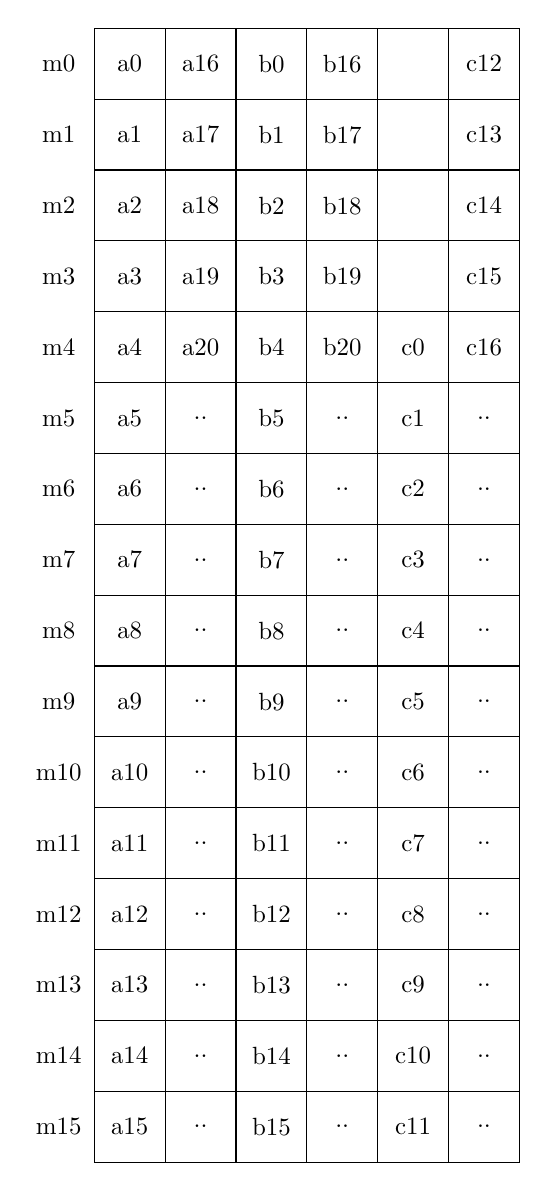
\begin{tikzpicture}[scale=0.9, transform shape]
	\tikzstyle{Element} = [draw=black, minimum width=1cm, minimum height=1cm, node distance=1cm]
	
	\node[name=m0]{m0};
	\node[name=m1, below of=m0]{m1};
	\node[name=m2, below of=m1]{m2};
	\node[name=m3, below of=m2]{m3};
	\node[name=m4, below of=m3]{m4};
	\node[name=m5, below of=m4]{m5};
	\node[name=m6, below of=m5]{m6};
	\node[name=m7, below of=m6]{m7};
	\node[name=m8, below of=m7]{m8};
	\node[name=m9, below of=m8]{m9};
	\node[name=m10, below of=m9]{m10};
	\node[name=m11, below of=m10]{m11};
	\node[name=m12, below of=m11]{m12};
	\node[name=m13, below of=m12]{m13};
	\node[name=m14, below of=m13]{m14};
	\node[name=m15, below of=m14]{m15};
	
	\node[name=a0, right of=m0, Element]{a0};
	\node[name=a1, below of=a0, Element]{a1};
	\node[name=a2, below of=a1, Element]{a2};
	\node[name=a3, below of=a2, Element]{a3};
	\node[name=a4, below of=a3, Element]{a4};
	\node[name=a5, below of=a4, Element]{a5};
	\node[name=a6, below of=a5, Element]{a6};
	\node[name=a7, below of=a6, Element]{a7};
	\node[name=a8, below of=a7, Element]{a8};
	\node[name=a9, below of=a8, Element]{a9};
	\node[name=a10, below of=a9, Element]{a10};
	\node[name=a11, below of=a10, Element]{a11};
	\node[name=a12, below of=a11, Element]{a12};
	\node[name=a13, below of=a12, Element]{a13};
	\node[name=a14, below of=a13, Element]{a14};
	\node[name=a15, below of=a14, Element]{a15};
	
	\node[name=a16, right of=a0, Element]{a16};
	\node[name=a17, below of=a16, Element]{a17};
	\node[name=a18, below of=a17, Element]{a18};
	\node[name=a19, below of=a18, Element]{a19};
	\node[name=a20, below of=a19, Element]{a20};
	\node[name=bl1, below of=a20, Element]{..};
	\node[name=bl2, below of=bl1, Element]{..};
	\node[name=bl3, below of=bl2, Element]{..};
	\node[name=bl4, below of=bl3, Element]{..};
	\node[name=bl5, below of=bl4, Element]{..};
	\node[name=bl6, below of=bl5, Element]{..};
	\node[name=bl7, below of=bl6, Element]{..};
	\node[name=bl8, below of=bl7, Element]{..};
	\node[name=bl9, below of=bl8, Element]{..};
	\node[name=bl10, below of=bl9, Element]{..};
	\node[name=bl11, below of=bl10, Element]{..};
	
	\node[name=b0, right of=a16, Element]{b0};
	\node[name=b1, below of=b0, Element]{b1};
	\node[name=b2, below of=b1, Element]{b2};
	\node[name=b3, below of=b2, Element]{b3};
	\node[name=b4, below of=b3, Element]{b4};
	\node[name=b5, below of=b4, Element]{b5};
	\node[name=b6, below of=b5, Element]{b6};
	\node[name=b7, below of=b6, Element]{b7};
	\node[name=b8, below of=b7, Element]{b8};
	\node[name=b9, below of=b8, Element]{b9};
	\node[name=b10, below of=b9, Element]{b10};
	\node[name=b11, below of=b10, Element]{b11};
	\node[name=b12, below of=b11, Element]{b12};
	\node[name=b13, below of=b12, Element]{b13};
	\node[name=b14, below of=b13, Element]{b14};
	\node[name=b15, below of=b14, Element]{b15};
	
	\node[name=b16, right of=b0, Element]{b16};
	\node[name=b17, below of=b16, Element]{b17};
	\node[name=b18, below of=b17, Element]{b18};
	\node[name=b19, below of=b18, Element]{b19};
	\node[name=b20, below of=b19, Element]{b20};
	\node[name=bl12, below of=b20, Element]{..};
	\node[name=bl13, below of=bl12, Element]{..};
	\node[name=bl14, below of=bl13, Element]{..};
	\node[name=bl15, below of=bl14, Element]{..};
	\node[name=bl16, below of=bl15, Element]{..};
	\node[name=bl17, below of=bl16, Element]{..};
	\node[name=bl18, below of=bl17, Element]{..};
	\node[name=bl19, below of=bl18, Element]{..};
	\node[name=bl20, below of=bl19, Element]{..};
	\node[name=bl21, below of=bl20, Element]{..};
	\node[name=bl22, below of=bl21, Element]{..};
	
	\node[name=bl23, right of=b16, Element]{};
	\node[name=bl24, below of=bl23, Element]{};
	\node[name=bl25, below of=bl24, Element]{};
	\node[name=bl26, below of=bl25, Element]{};
	\node[name=c1, below of=bl26, Element]{c0};
	\node[name=c2, below of=c1, Element]{c1};
	\node[name=c3, below of=c2, Element]{c2};
	\node[name=c4, below of=c3, Element]{c3};
	\node[name=c5, below of=c4, Element]{c4};
	\node[name=c6, below of=c5, Element]{c5};
	\node[name=c7, below of=c6, Element]{c6};
	\node[name=c8, below of=c7, Element]{c7};
	\node[name=c9, below of=c8, Element]{c8};
	\node[name=c10, below of=c9, Element]{c9};
	\node[name=c11, below of=c10, Element]{c10};
	\node[name=c12, below of=c11, Element]{c11};
	
	\node[name=c13, right of=bl23, Element]{c12};
	\node[name=c14, below of=c13, Element]{c13};
	\node[name=c15, below of=c14, Element]{c14};
	\node[name=c16, below of=c15, Element]{c15};
	\node[name=c17, below of=c16, Element]{c16};
	\node[name=c18, below of=c17, Element]{..};
	\node[name=c19, below of=c18, Element]{..};
	\node[name=c20, below of=c19, Element]{..};
	\node[name=bl27, below of=c20, Element]{..};
	\node[name=bl28, below of=bl27, Element]{..};
	\node[name=bl29, below of=bl28, Element]{..};
	\node[name=bl30, below of=bl29, Element]{..};
	\node[name=bl31, below of=bl30, Element]{..};
	\node[name=bl32, below of=bl31, Element]{..};
	\node[name=bl33, below of=bl32, Element]{..};
	\node[name=bl34, below of=bl33, Element]{..};
\end{tikzpicture}
\end{center}

\begin{figure}
\includegraphics[scale=0.7]{coordinate.png}
\caption{Time slot 0 - 16}
\end{figure}

\begin{figure}
\includegraphics[scale=0.7]{coordinate2.png}
\caption{Time slot 16 - 33}
\end{figure}

\subsection{If there are any conflicts during the operation identify them and illustrate how in this specific case you will avoid the conflicts(if there are any).}

\begin{doublespace}
In this case, we can only fetch $b_{i}$ after $a_{i}$ being fetched, so it is required to buffer $a_{i}$ two cycles. We have to introduce  delay element in input stream A.\\
Due to storing $c_{i}$ smartly 4 modules away, the writing conflict is avoid, so it is no need to introduce any delay element to output.
\end{doublespace}
\end{document}